\documentclass[a4paper,14pt]{extarticle}
\usepackage[margin=20pt]{geometry}
\usepackage[french]{babel}
\usepackage[utf8]{inputenc}
\usepackage[T1]{fontenc}
\usepackage{graphicx}
\usepackage[export]{adjustbox}
\graphicspath{ {./images/} }
\usepackage{amsmath}
\usepackage{amsfonts}
\usepackage{amssymb}
\usepackage{mathrsfs}
\usepackage[shortlabels]{enumitem}
\usepackage[version=4]{mhchem}
\usepackage{stmaryrd}
\usepackage[default,oldstyle,scale=0.95]{opensans}

\setlistdepth{9}

\setlist[itemize,1]{label=$\bullet$}
\setlist[itemize,2]{label=$\bullet$}
\setlist[itemize,3]{label=$\bullet$}
\setlist[itemize,4]{label=$\bullet$}
\setlist[itemize,5]{label=$\bullet$}
\setlist[itemize,6]{label=$\bullet$}
\setlist[itemize,7]{label=$\bullet$}
\setlist[itemize,8]{label=$\bullet$}
\setlist[itemize,9]{label=$\bullet$}

\renewlist{itemize}{itemize}{9}

\title{DIPLÔME NATIONAL DU BREVET SESSION 2024 }

\author{}
\date{}


\begin{document}
% \maketitle
\vspace{.4\textheight}
\parbox[b]{0.75\textwidth}{
 {\Large\bfseries DIPLÔME NATIONAL DU BREVET }\\[0.5\baselineskip]
 {\Large\bfseries SESSION 2024 }\\[4\baselineskip]
 \large MATHEMATIQUES \\[0.5\baselineskip]
 \large Série générale \\[2\baselineskip]
 \normalsize Durée de l'épreuve: 2 h 00 \\[0.5\baselineskip]
 \normalsize 100 points \\[2\baselineskip]
 }

Dès que le sujet vous est remis, assurez-vous qu'il est complet.
Il comporte 6 pages numérotées de la page 1 sur 6 à la page 6 sur 6 .
L'usage de la calculatrice avec mode examen actif est autorisé 
L'usage de la calculatrice sans mémoire «type collège » est autorisé
L'utilisation du dictionnaire est interdite.

\begin{center}
\begin{tabular}{|c|c|}
\hline
Exercice 1 & 20 points \\
\hline
Exercice 2 & 20 points \\
\hline
Exercice 3 & 22 points \\
\hline
Exercice 4 & 18 points \\
\hline
Exercice 5 & 20 points \\
\hline
\end{tabular}
\end{center}

\newpage

\section*{Indications portant sur l'ensemble du sujet.}
Toutes les réponses doivent être justifiées, sauf si une indication contraire est donnée. Pour chaque question, si le travail n'est pas terminé, laisser tout de même une trace de la recherche ; elle sera prise en compte dans la notation.

\section*{Exercice 1 (20 points)}
Au casino, la roulette est un jeu de hasard pour lequel chaque joueur mise au choix sur un ou plusieurs numéros. On lance une bille sur une roue qui tourne, numérotée de 0 à 36 .

La bille a la même probabilité de s'arrêter sur chaque numéro.

\begin{center}
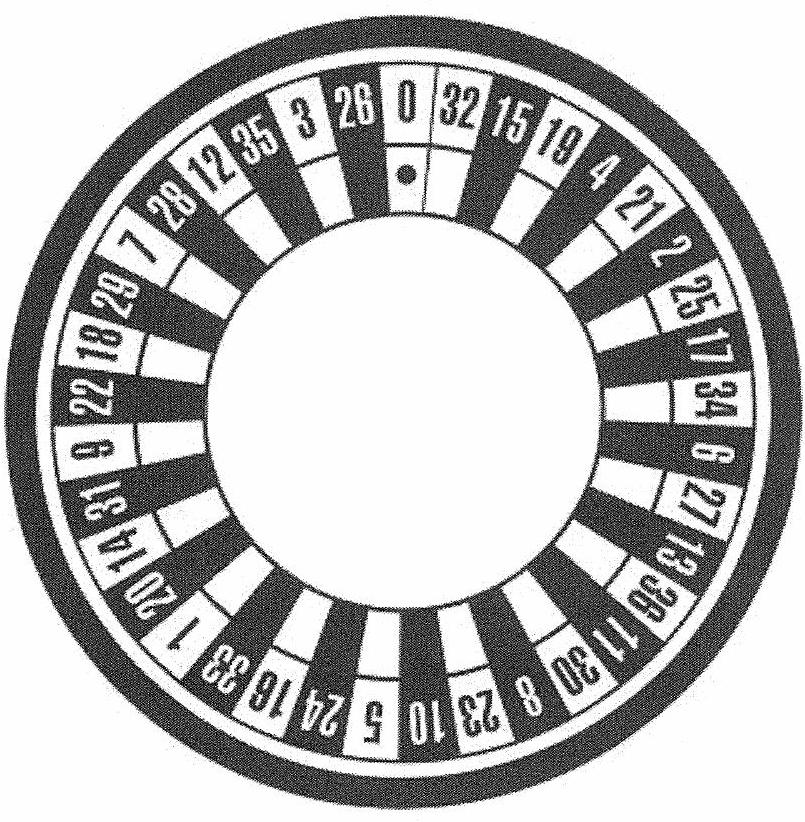
\includegraphics[max width=0.4\textwidth]{ex1}
\end{center}

\begin{enumerate}
  \item Expliquer pourquoi la probabilité que la bille s'arrête sur le numéro 7 est $\frac{1}{37}$.

  \item Déterminer la probabilité que la bille s'arrête sur une case à la fois noire et paire.

  \item \begin{enumerate}[a.] 
      \item Déterminer la probabilité que la bille s'arrête sur un numéro inférieur ou égal à 6 .

      \item En déduire la probabilité que la bille s'arrête sur un numéro supérieur ou égal à 7 .

      \item Un joueur affirme qu'on a plus de 3 chances sur 4 d'obtenir un numéro supérieur ou égal à 7 . A-t-il raison ?
        
    \end{enumerate}
\end{enumerate}
\newpage
\section*{Exercice 2 (20 points)}
\begin{tabular}{|c|c|}
\hline
Programme A & Programme B \\
\hline
\begin{tabular}[t!]{@{}l@{}}
- Choisir un nombre.\\
- Prendre le carré du nombre choisi.\\
- Multiplier le résultat par 2.\\
- Ajouter le double du nombre de départ. \\
- Soustraire 4 au résultat. \\
\end{tabular} & \raisebox{-3cm}{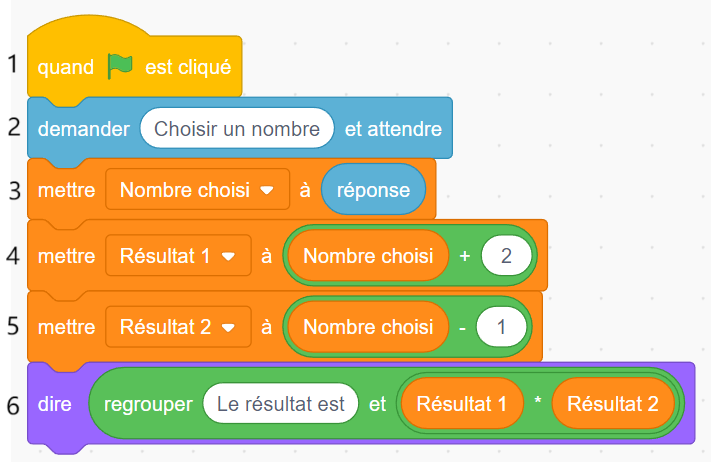
\includegraphics[max width=.45\textwidth]{scratch} }\\
\hline
\end{tabular}
\begin{enumerate}

  \item \begin{enumerate}[a.] 
    \item Vérifier que, si on choisit 5 comme nombre de départ, le résultat du programme A est 56 .

    \item Quel résultat obtient-on avec le programme $B$ si on choisit -9 comme nombre de départ?

    \end{enumerate}

  \item On choisit un nombre quelconque $x$ comme nombre de départ.
    \begin{enumerate}[a.] 

      \item Parmi les trois propositions ci-dessous, recopier l'expression qui donne le résultat obtenu par le programme B ?

        $$
        E_{1}=(x+2)-1 \quad E_{2}=(x+2) \times(x-1) \quad E_{3}=x+2 \times x-1
        $$

      \item Exprimer en fonction de $x$ le résultat obtenu avec le programme $\mathrm{A}$

    \end{enumerate}
  \item Démontrer que, quel que soit le nombre choisi au départ, le résultat du programme A est toujours le double du résultat du programme B.
\end{enumerate}
\newpage
\section*{Exercice 3 (22 points)}
Sur la figure ci-dessous, on a :

\begin{itemize}
  \item $\mathscr{C}$ est un cercle de centre O et de rayon 4,5cm;
  \item [AB] est un diamètre de ce cercle et D est un point du cercle ;
  \item les points B, E, A sont alignés, ainsi que les points D, F, A;
  \item les droites (BD) et (EF) sont parallèles ;
  \item BD = 5,4 cm ; DA = 7,2 cm et AE = 2,7 cm.
\end{itemize}

\begin{center}
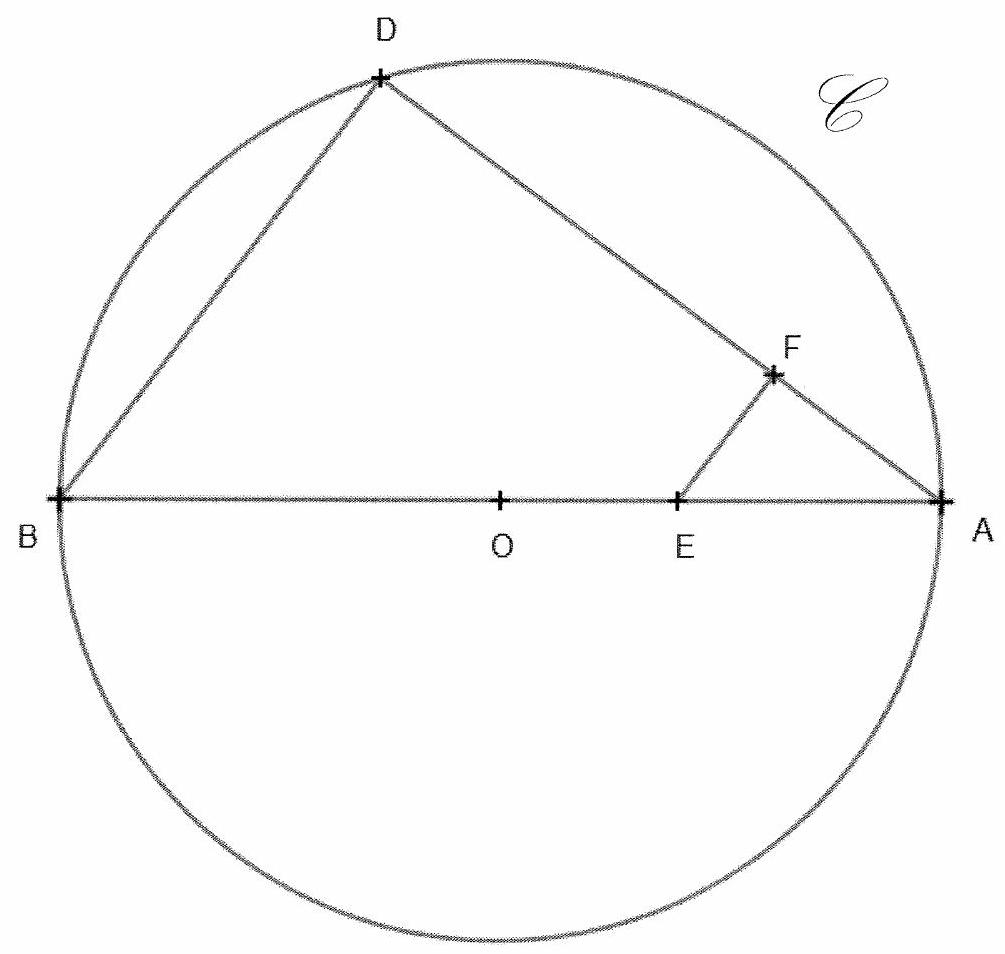
\includegraphics[max width=.5\textwidth]{ex3}
\end{center}

\begin{enumerate}
  \item Justifier que le diamètre [AB] mesure 9 cm.

  \item Démontrer que le triangle ABD est rectangle en D.

  \item Calculer AF.
  \item \begin{enumerate}[a.]
    \item Justifier que l'aire du triangle ABD est égale à 19,44 cm².

    \item Calculer l'aire du disque, arrondie au centième.

    Rappel : l'aire du disque est égale à $\pi \times R^{2}$, où $R$ est le rayon du disque.

    \end{enumerate}

  \item Quel pourcentage de l'aire du disque représente l'aire du triangle ABD ?
\end{enumerate}
\newpage
\section*{Exercice 4 (18 points)}
Cet exercice est un questionnaire à choix multiple (QCM). Pour chaque question, trois réponses (A, B ou $\mathrm{C}$ ) sont proposées. Une seule réponse est exacte. Recopier sur la copie le numéro de la question et la lettre correspondant à la réponse exacte. Aucune justification n'est demandée.

\begin{center}
\begin{tabular}{|l|c|c|c|}
  Question & Réponse A & Réponse B & Réponse C \\
  \hline
  \begin{tabular}{@{}l@{}} \textbf{1.} On considère la fonction $f$ définie par \\ $f(x)=3x-2$ \\ Quelle est l'image de -4 par cette fonction? \end{tabular}& -14 & -10 & -3\\
  \hline
  \textbf{2.} Combien vaut (-5)³ ? & -125 & -15 & 125 \\
  \hline
  \begin{tabular}{@{}l@{}} \textbf{3.} Quelle est l'image de la translation du point J \\ par la translation qui transforme C en A ? \\ 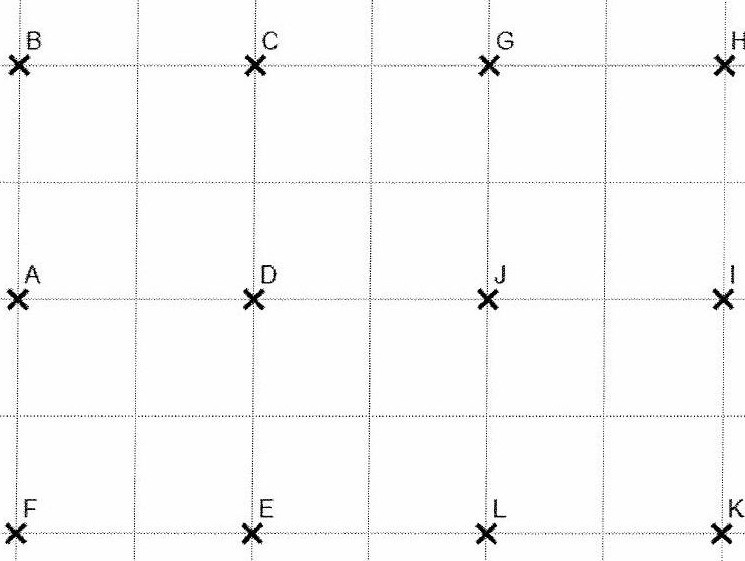
\includegraphics[max width=.3\textwidth]{qcm3}\end{tabular} & H & E & D\\
  \hline
  \begin{tabular}{@{}l@{}} \textbf{4.} Quel est l'antécédent de 3 par la fonction $f$? \\ 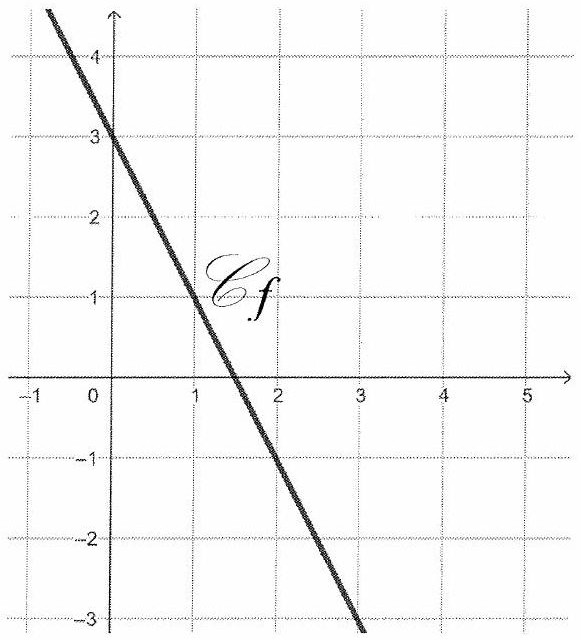
\includegraphics[max width=.3\textwidth]{qcm4}\end{tabular} & 3 & -3 & 0\\
  \hline
  \begin{tabular}{@{}l@{}} \textbf{5.} On a mesuré les tailles, en m, de sept élèves :\\ 1,46 ; 1,65 ; 1,6 ; 1,72 ; 1,7 ; 1,67 ; 1,75 \\ Quelle est la médiane, en m, de ces tailles? \end{tabular} & 0,8 & 0,75 & 0,6 \\
  \hline 
\end{tabular}
\end{center}
\newpage
\section*{Exercice 5 (20 points)}
Un club de natation propose un après-midi découverte pour les enfants.

\section*{PARTIE A}
La présidente du club veut offrir des petits sachets cadeaux tous identiques contenant des autocollants et des drapeaux avec le logo du club. Elle a acheté 330 autocollants et 132 drapeaux et veut tous les utiliser. Elle veut que, dans chaque sachet, il y ait exactement le même nombre d'autocollants et que, dans chaque sachet, il y ait exactement le même nombre de drapeaux.

\begin{enumerate}[1.]
  \item Pourquoi n'est-il pas possible de faire 15 sachets ?

  \item  \begin{enumerate}[a.] 

    \item Décomposer 330 et 132 en produits de facteurs premiers.

    \item En déduire le plus grand nombre de sachets que la présidente pourra réaliser.

    \item Dans ce cas, combien mettra-t-elle d'autocollants et de drapeaux dans chaque sachet ?
  \end{enumerate}
\end{enumerate}

\section*{PARTIE B}
La piscine a la forme d'un pavé droit représenté ci-dessous.

Elle est remplie aux $\frac{9}{10}$ du volume.

$1 \mathrm{~m}^{3}$ d'eau coûte $4,14$ €.

Combien coûte le remplissage de la piscine ?

\begin{center}
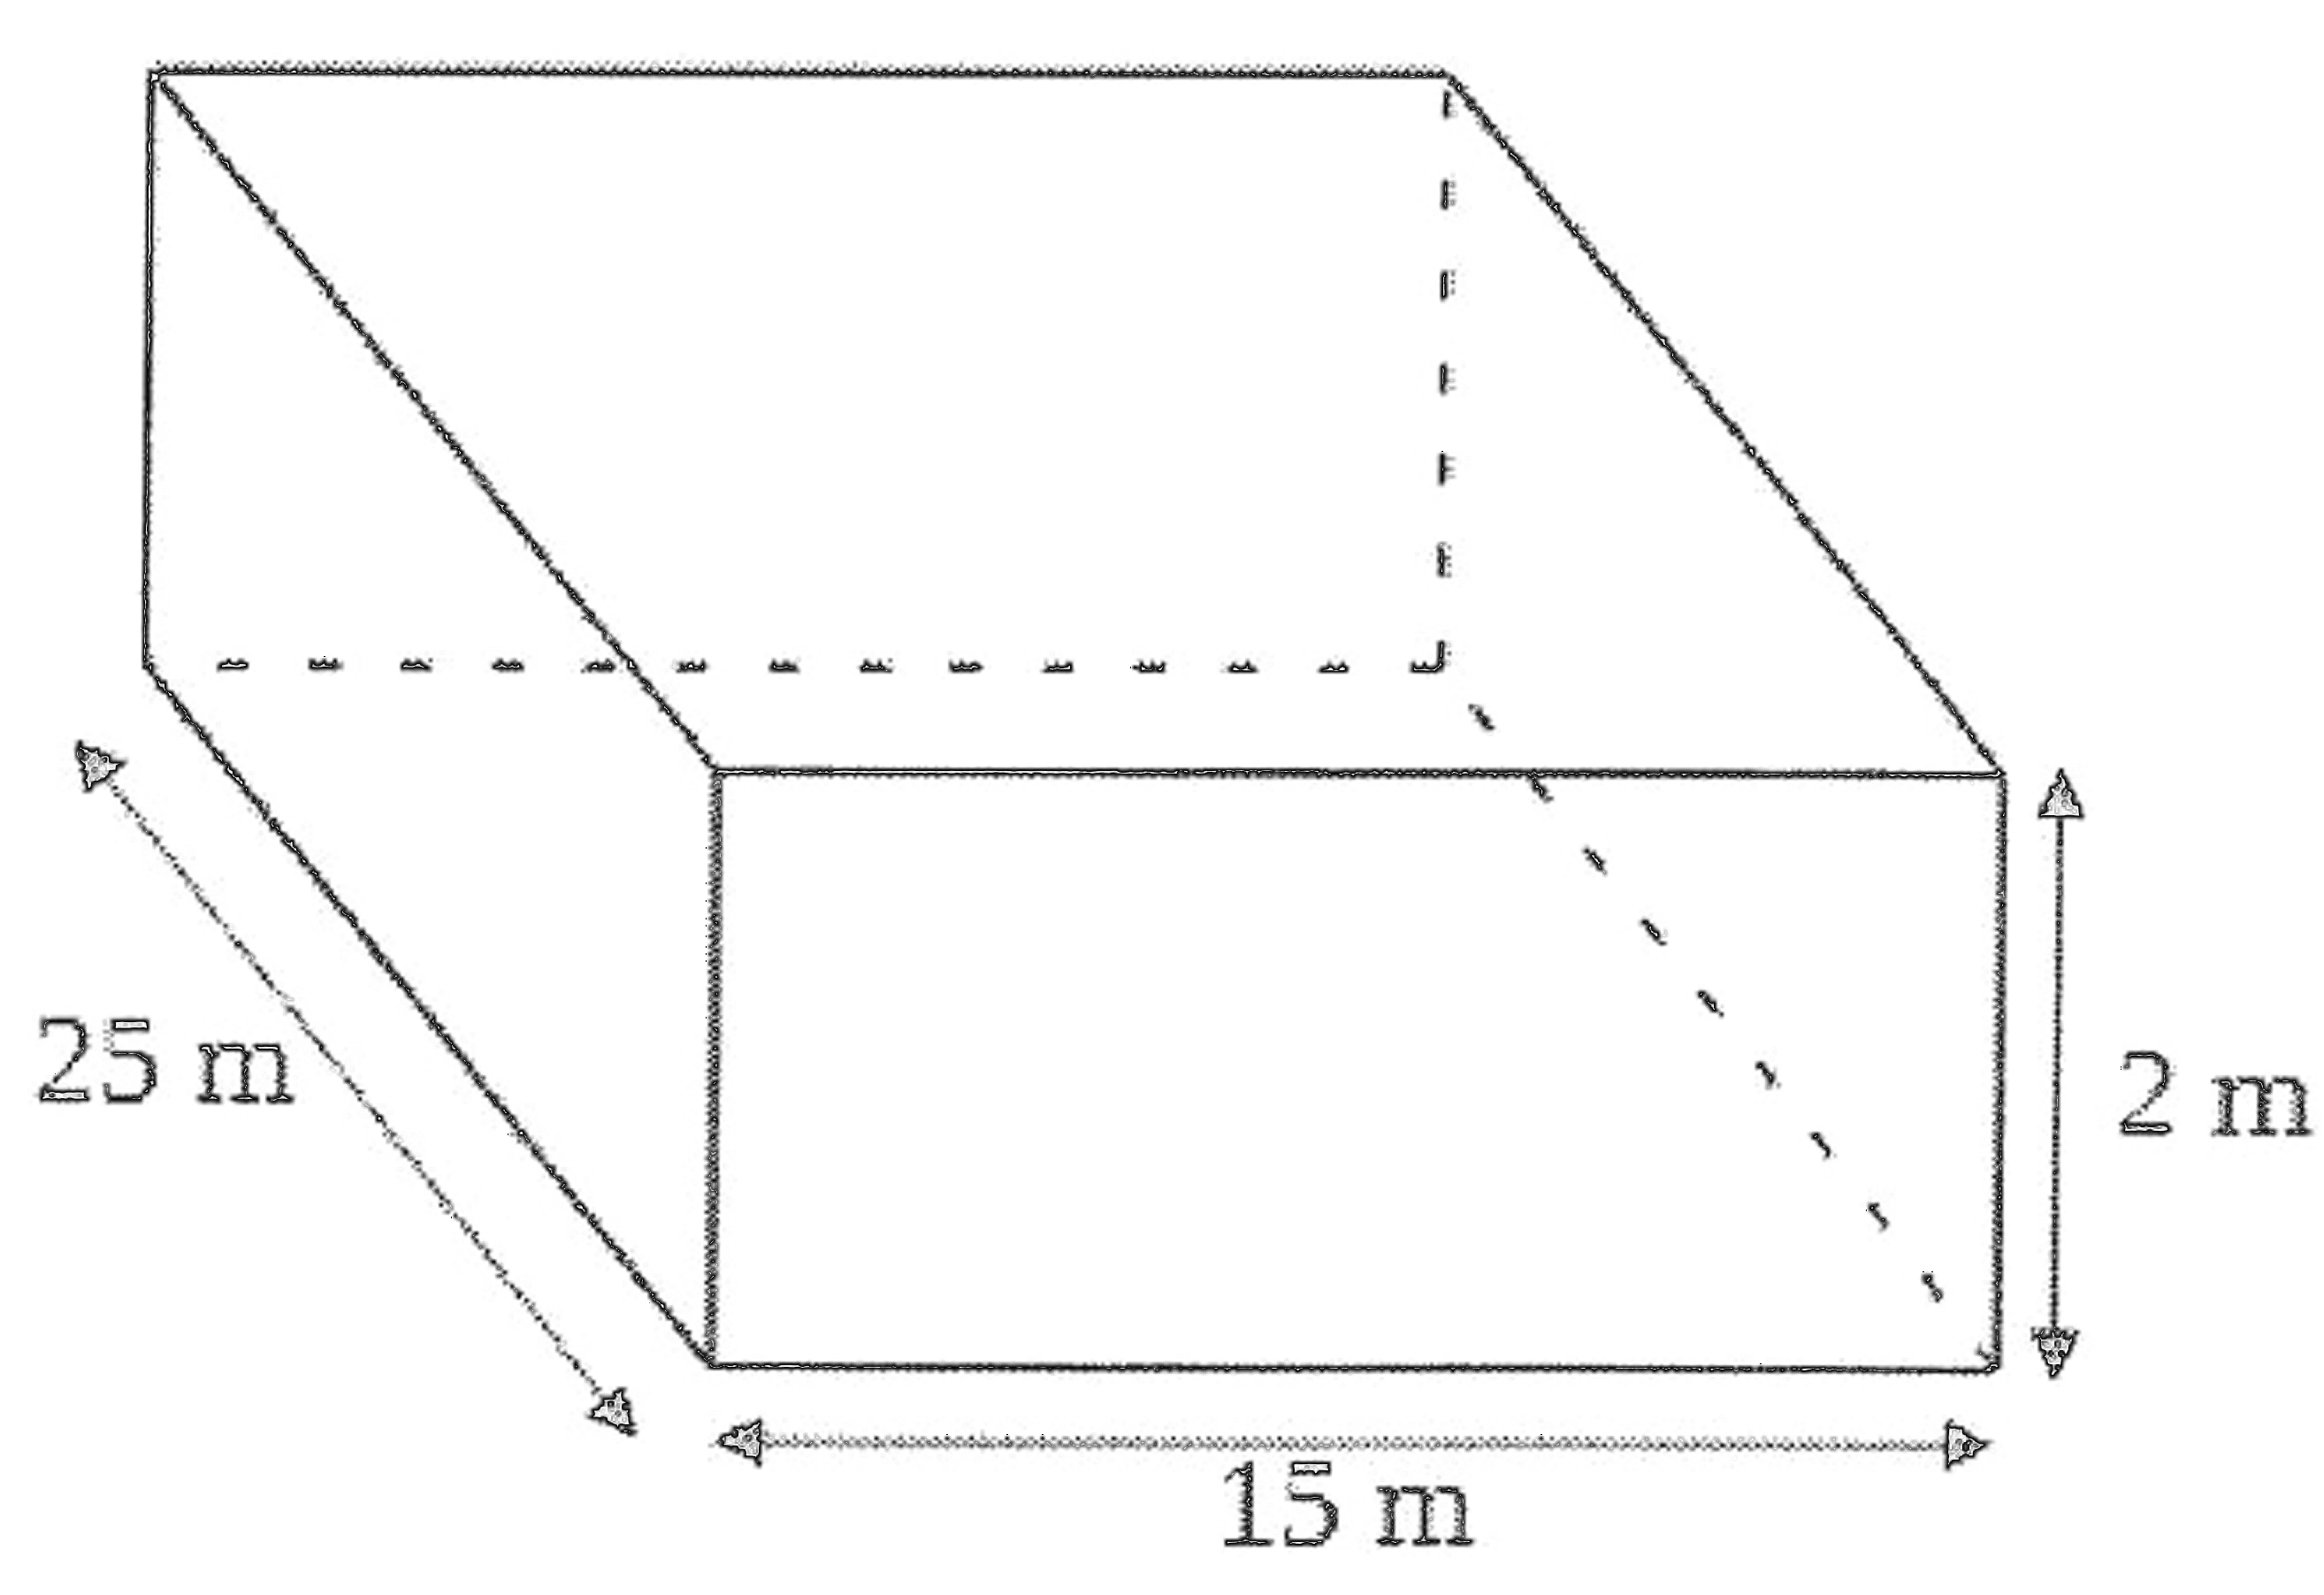
\includegraphics[max width=.5\textwidth]{piscine}
\end{center}


\end{document}